\subsection{FT Properties}
\begin{definition}
    We denote the Fourier Transform pair as:
    \[
    x(t) \overset{F}{\leftrightarrow} X(f)
    \]
    \vspace{1em}

    \textbf{Fourier Transform:}
    \[
    X(f) = \int_{-\infty}^{\infty} x(t) e^{-j 2 \pi f t} \, dt
    \]
    \[
    x(t) = \int_{-\infty}^{\infty} X(f) e^{j 2 \pi f t} \, df
    \]
    \vspace{1em}

    \textbf{Fourier Transform Conventions}
    \begin{itemize}
        \item Use lowercase letters for time domain functions (e.g., \( x(t) \)).
        \item Use uppercase letters for frequency domain functions (e.g., \( X(f) \)).
    \end{itemize}
\end{definition}

\subsubsection{Common Fourier Transform Pairs}
\begin{definition}
    \begin{enumerate}
    \item For the rectangular function:
    \[
    \text{rect}(t) \overset{F}{\leftrightarrow} \text{sinc}(f)
    \]
    \customFigure[0.75]{00_Images/RECT3.png}{Time domain to frequency domain.}

    \item For \( x(t) = e^{-at} u(t) \):
    \begin{equation*}
        e^{-at} u(t) \overset{F}{\leftrightarrow} \frac{1}{a + j 2 \pi f} \text{ for $a > 0$}
    \end{equation*}
    \begin{itemize}
        \item \textbf{Proof:} \begin{align*}
            X(f) &= \int_{0}^{\infty} e^{-at} e^{-j 2 \pi f t} \, dt \\
                &= \left. \frac{e^{-(a + j 2 \pi f)t}}{-(a + j 2 \pi f)} \right|_0^{\infty} = \frac{1}{a + j 2 \pi f} \quad \text{for } a > 0
        \end{align*}
    \end{itemize}

    \item For \( x(t) = \delta(t) \):
    \begin{equation*}
        \delta(t) \overset{F}{\leftrightarrow} 1 
    \end{equation*}
    \begin{itemize}
        \item \textbf{Proof:} $X(f) = \int_{-\infty}^{\infty} \delta(t) e^{-j 2 \pi f t} \, dt =  \int_{-\infty}^{\infty} \delta(t) e^{j0} \, dt = 1$
    \end{itemize}

    \item For \( X(f) = \delta(f) \):
    \begin{equation*}
        1 \overset{F}{\leftrightarrow} \delta(f)
    \end{equation*}
    \begin{itemize}
        \item \textbf{Proof:} $x(t) = \int_{-\infty}^{\infty} \delta(f) e^{j 2 \pi f t} \, df = \int_{-\infty}^{\infty} \delta(f) e^{j 0} \, df = 1$
    \end{itemize}

    \item For \( x(t) = \delta(t - t_0) \):
    \begin{equation*}
        \delta(t - t_0) \overset{F}{\leftrightarrow} e^{-j 2 \pi f t_0} 
    \end{equation*}
    \begin{itemize}
        \item \textbf{Proof:} $X(f) = \int_{-\infty}^{\infty} \delta(t - t_0) e^{-j 2 \pi f t} \, dt = e^{-j 2 \pi f t_0}$
    \end{itemize}
    \customFigure[0.5]{00_Images/P1.png}{.}

    \item For \( X(f) = \delta(f - f_0) \):
    \begin{equation*}
        e^{j 2 \pi f_0 t} \overset{F}{\leftrightarrow} \delta(f - f_0)
    \end{equation*}
    \begin{itemize}
        \item \textbf{Proof:} $x(t) = \int_{-\infty}^{\infty} \delta(f - f_0) e^{j 2 \pi f t} \, df = e^{j 2 \pi f_0 t}$
    \end{itemize}
    \customFigure[0.5]{00_Images/P2.png}{.}

    \item \textbf{Linearity property:} If \( x \overset{F}{\leftrightarrow} X \) and \( y \overset{F}{\leftrightarrow} Y \), then
    \[
    \alpha x + \beta y \overset{F}{\leftrightarrow} \alpha X + \beta Y \quad \text{for all } \alpha, \beta \in \mathbb{C}
    \]
    \begin{itemize}
        \item \textbf{Proof:}
        \begin{align*}
            \int_{-\infty}^{\infty} \left( \alpha x(t) + \beta y(t) \right) e^{-j 2 \pi f t} \, dt &= \alpha \int_{-\infty}^{\infty} x(t) e^{-j 2 \pi f t} \, dt + \beta \int_{-\infty}^{\infty} y(t) e^{-j 2 \pi f t} \, dt \\
            &= \alpha X + \beta Y
        \end{align*}
    \end{itemize}
    \item \textbf{General linearity property:} 
    \[
    \sum_{k \in \mathbb{Z}} \alpha_k x_k \overset{F}{\leftrightarrow} \sum_{k \in \mathbb{Z}} \alpha_k X_k
    \]
    \end{enumerate}
\end{definition}

\subsection{Fourier Series Transforms of Periodic Signals (4.2)}
\begin{definition}
    Suppose \( x \underset{T}{\overset{FS}{\leftrightarrow}} c_k \), then
    \[
    x(t) = \sum_{k \in \mathbb{Z}} c_k e^{j 2 \pi \frac{k}{T} t} \rightarrow X(f) = \sum_{k \in \mathbb{Z}} c_k \delta\left(f - \frac{k}{T}\right) \quad \text{(Line Spectrum)}
    \]
    \begin{itemize}
        \item i.e. Periodic signals have a line spectrum as the Fourier Transform.
    \end{itemize}
\end{definition}

\begin{example}
    \begin{enumerate}
        \item For \( x(t) = \cos(2 \pi f_0 t) \):
           \begin{align*}
               x(t) &= \frac{1}{2} e^{j 2 \pi f_0 t} + \frac{1}{2} e^{-j 2 \pi f_0 t} \\
               X(f) &= \frac{1}{2} \delta(f - f_0) + \frac{1}{2} \delta(f + f_0)
           \end{align*}
           \customFigure[0.5]{00_Images/COS.png}{.}
        
        \item For \( y(t) = \sin(2 \pi f_0 t) \):
           \begin{align*}
               y(t) &= \frac{1}{2j} e^{j 2 \pi f_0 t} - \frac{1}{2j} e^{-j 2 \pi f_0 t} \\
               X(f) &= \frac{1}{2j} \delta(f - f_0) - \frac{1}{2j} \delta(f + f_0)
           \end{align*}
           \customFigure[0.5]{00_Images/SINE.png}{.}
        
        \item For the periodic rectangle function.
        \[
        x(t) \underset{T}{\overset{FS}{\longleftrightarrow}} c_k = \frac{1}{T} \, \text{sinc} \left( \frac{k}{T} \right)
        \]
        \customFigure[0.5]{00_Images/RECT4.png}{.}
        \[
        X(f) = \sum_{k \in \mathbb{Z}} \frac{1}{T} \, \text{sinc} \left( \frac{k}{T} \right) \delta \left( f - \frac{k}{T} \right)
        \]
        \customFigure[0.5]{00_Images/REC5.png}{Also a line spectrum (note, in reality these lines diverge to infinity, but we have just drawn in this manner to scale the area to $1$)}

        \item For the rectangular pulse train:
           \[
           x(t) = \sum_{k \in \mathbb{Z}} \delta(t - kT) \underset{T}{\overset{FS}{\longleftrightarrow}} c_k = \frac{1}{T}
           \]
           \[
           X(f) = \sum_{k \in \mathbb{Z}} \frac{1}{T} \delta\left(f - \frac{k}{T}\right)
           \]
           This represents a \textbf{picket fence function}, which will be significant in sampling theory.
           \customFigure[0.75]{00_Images/PF.png}{Picket fence.}
           \begin{itemize}
            \item \textbf{Reciprocal Spacing:} If the spacing is wide in the time domain, then the spacing will be narrow in the frequency domain. Vice versa.
           \end{itemize}
    \end{enumerate}
\end{example}

\subsection{Properties of Fourier Transform (MIDTERM CUTOFF EXCLUSIVE)}
\begin{warning}
    \begin{itemize}
        \item Time domain is on left side of FT Pair and frequency domain is on the right side.
    \end{itemize}
\end{warning}

\subsubsection{1. Linearity}
\begin{definition}
    If \( x(t) \overset{\mathcal{F}}{\leftrightarrow} X(f) \) and \( y(t) \overset{\mathcal{F}}{\leftrightarrow} Y(f) \), then
\[
\alpha x(t) + \beta y(t) \overset{\mathcal{F}}{\leftrightarrow} \alpha X(f) + \beta Y(f), \quad \forall \, \alpha, \beta \in \mathbb{C}.
\]
\end{definition}

\subsubsection{2. Time-shifting}
\begin{definition}
    If \( x(t) \overset{\mathcal{F}}{\leftrightarrow} X(f) \), then
\[
x(t - t_0) \overset{\mathcal{F}}{\leftrightarrow} e^{-j 2 \pi f t_0} X(f).
\]
\end{definition}

\begin{derivation}
    \textbf{Proof:}
    \begin{align*}
    \mathcal{F}^{-1} \left( e^{-j 2 \pi f t_0} X(f) \right) &= \int_{-\infty}^{\infty} X(f) e^{-j 2 \pi f t_0} e^{j 2 \pi f t} \, df \\
    &= \int_{-\infty}^{\infty} X(f) e^{j 2 \pi f (t - t_0)} \, df \\
    &= x(t - t_0).
    \end{align*}
\end{derivation}

\subsubsection{3. Frequency-shifting (Modulation)}
\begin{definition}
    If \( x(t) \overset{\mathcal{F}}{\leftrightarrow} X(f) \), then
    \[
    e^{j 2 \pi f_0 t} x(t) \overset{\mathcal{F}}{\leftrightarrow} X(f - f_0).
    \]
\end{definition}

\begin{derivation}
    \textbf{Proof:}
    \begin{align*}
    \mathcal{F} \left( e^{j 2 \pi f_0 t} x(t) \right) &= \int_{-\infty}^{\infty} e^{j 2 \pi f_0 t} x(t) e^{-j 2 \pi f t} \, dt \\
    &= \int_{-\infty}^{\infty} x(t) e^{-j 2 \pi (f - f_0) t} \, dt \\
    &= X(f - f_0).
    \end{align*}
\end{derivation}

\subsubsection{4. Time-reversal}
\begin{definition}
    If \( x(t) \overset{\mathcal{F}}{\leftrightarrow} X(f) \), then
    \[
    \tilde{x}(t) = x(-t) \overset{\mathcal{F}}{\leftrightarrow} \tilde{X}(f) = X(-f).
    \]
\end{definition}

\begin{derivation}
    \textbf{Proof:}
    \begin{align*}
    \mathcal{F} \left( x(-t) \right) &= \int_{-\infty}^{\infty} x(-t) e^{-j 2 \pi f t} \, dt \\
    &= \int_{\infty}^{-\infty} x(s) e^{-j 2 \pi f (-s)} (-ds) \quad \text{(substitute } s = -t, \, ds = -dt) \\
    &= \int_{-\infty}^{\infty} x(s) e^{-j 2 \pi (-f) s} \, ds \\
    &= X(-f) \\
    &= \tilde{X}(f).
    \end{align*}
\end{derivation}

\subsubsection{5. Conjugation}
\begin{definition}
    If \( x(t) \overset{\mathcal{F}}{\leftrightarrow} X(f) \), then
    \[
    x^*(t) \overset{\mathcal{F}}{\leftrightarrow} \tilde{X}^*(f) = X^*(-f).
    \]
\end{definition}

\begin{derivation}
    \textbf{Proof:}
    \begin{align*}
    \mathcal{F} \left( x^*(t) \right) &= \int_{-\infty}^{\infty} x^*(t) e^{-j 2 \pi f t} \, dt \\
    &= \left( \int_{-\infty}^{\infty} x(t) e^{j 2 \pi f t} \, dt \right)^* \\
    &= \left( \int_{-\infty}^{\infty} x(t) e^{-j 2 \pi (-f) t} \, dt \right)^* \\
    &= \left( X(-f) \right)^* \\
    &= X^*(-f).
    \end{align*}
\end{derivation}

\subsubsection{6. Duality}
\begin{definition}
    If \( x(t) \overset{\mathcal{F}}{\leftrightarrow} X(f) \), then
    \[
    X(t) \overset{\mathcal{F}}{\leftrightarrow} \tilde{x}(f) = x(-f).
    \]
\end{definition}

\begin{derivation}
    \textbf{Proof:}
    \begin{align*}
    X(f) &= \int_{-\infty}^{\infty} x(t) e^{-j 2 \pi f t} \, dt, \\
    X(t) &= \int_{-\infty}^{\infty} x(s) e^{-j 2 \pi t s} \, ds, \quad (t \rightarrow s) \text{ and } (f \rightarrow t) \\
    \mathcal{F}(X(t)) &= \int_{-\infty}^{\infty} X(t) e^{-j 2 \pi f t} \, dt \\
    &= \int_{-\infty}^{\infty} \left( \int_{-\infty}^{\infty} x(s) e^{-j 2 \pi t s} \, ds \right) e^{-j 2 \pi f t} \, dt \\
    &= \int_{-\infty}^{\infty} x(s) \int_{-\infty}^{\infty} e^{-j 2 \pi t s}  e^{-j 2 \pi f t} \, dt \, ds \\
    &= \int_{-\infty}^{\infty} x(s) \delta(s + f) \, ds \\
    &= x(-f) \\
    &= \tilde{x}(f)
    \end{align*}
\end{derivation}

\begin{figure}[h!]
    \centering
    % Left Diagram
    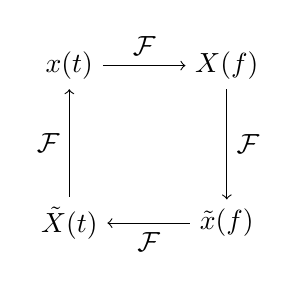
\begin{tikzpicture}
        % Nodes
        \node (X) at (0, 2) {\( x(t) \)};
        \node (XF) at (2, 2) {\( X(f) \)};
        \node (XTildeF) at (2, 0) {\( \tilde{x}(f) \)};
        \node (XTilde) at (0, 0) {\( \tilde{X}(t) \)};

        % Arrows
        \draw[->] (X) -- node[above] {\( \mathcal{F} \)} (XF);
        \draw[<-] (XTilde) -- node[below] {\( \mathcal{F} \)} (XTildeF);
        \draw[<-] (X) -- node[left] {\( \mathcal{F} \)} (XTilde);
        \draw[->] (XF) -- node[right] {\( \mathcal{F} \)} (XTildeF);
    \end{tikzpicture}
    \quad
    % Right Diagram
    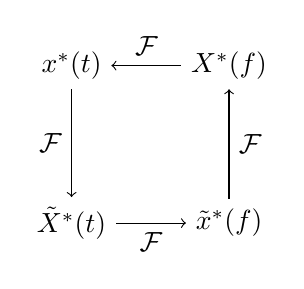
\begin{tikzpicture}
        % Nodes
        \node (XStar) at (0, 2) {\( x^*(t) \)};
        \node (XFStar) at (2, 2) {\( X^*(f) \)};
        \node (XTildeFStar) at (2, 0) {\( \tilde{x}^*(f) \)};
        \node (XTildeStar) at (0, 0) {\( \tilde{X}^*(t) \)};

        % Arrows
        \draw[<-] (XStar) -- node[above] {\( \mathcal{F} \)} (XFStar);
        \draw[->] (XTildeStar) -- node[below] {\( \mathcal{F} \)} (XTildeFStar);
        \draw[->] (XStar) -- node[left] {\( \mathcal{F} \)} (XTildeStar);
        \draw[<-] (XFStar) -- node[right] {\( \mathcal{F} \)} (XTildeFStar);
    \end{tikzpicture}
\end{figure}

